\chapter{球員}
\section{繪圖}
\newpage

\section{組裝}
\begin{figure}[hbt!]
  \begin{center}
    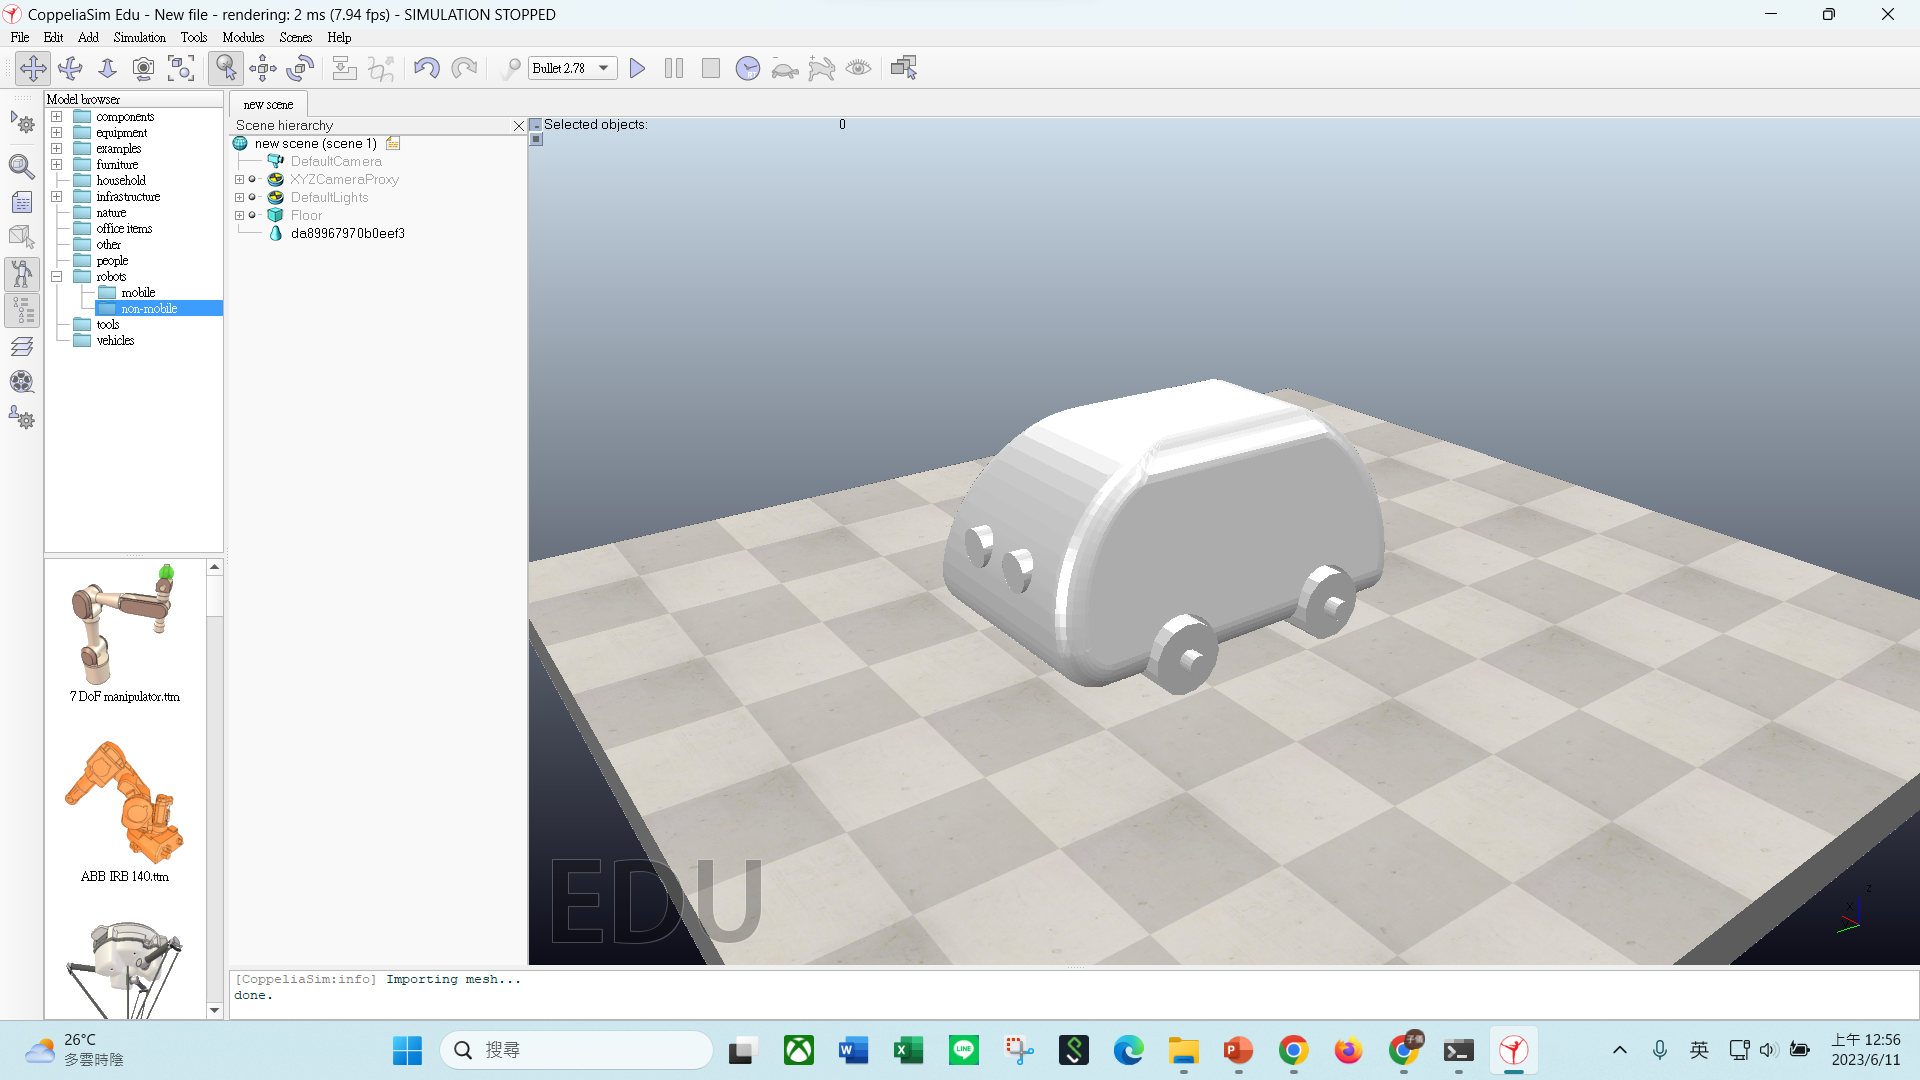
\includegraphics[width=0.5\textwidth]{球員組裝_1.png}
  \end{center}
  \caption{導入球員STL檔}
  \label{fig:photo}
\end{figure}

\begin{figure}[hbt!]
  \begin{center}
    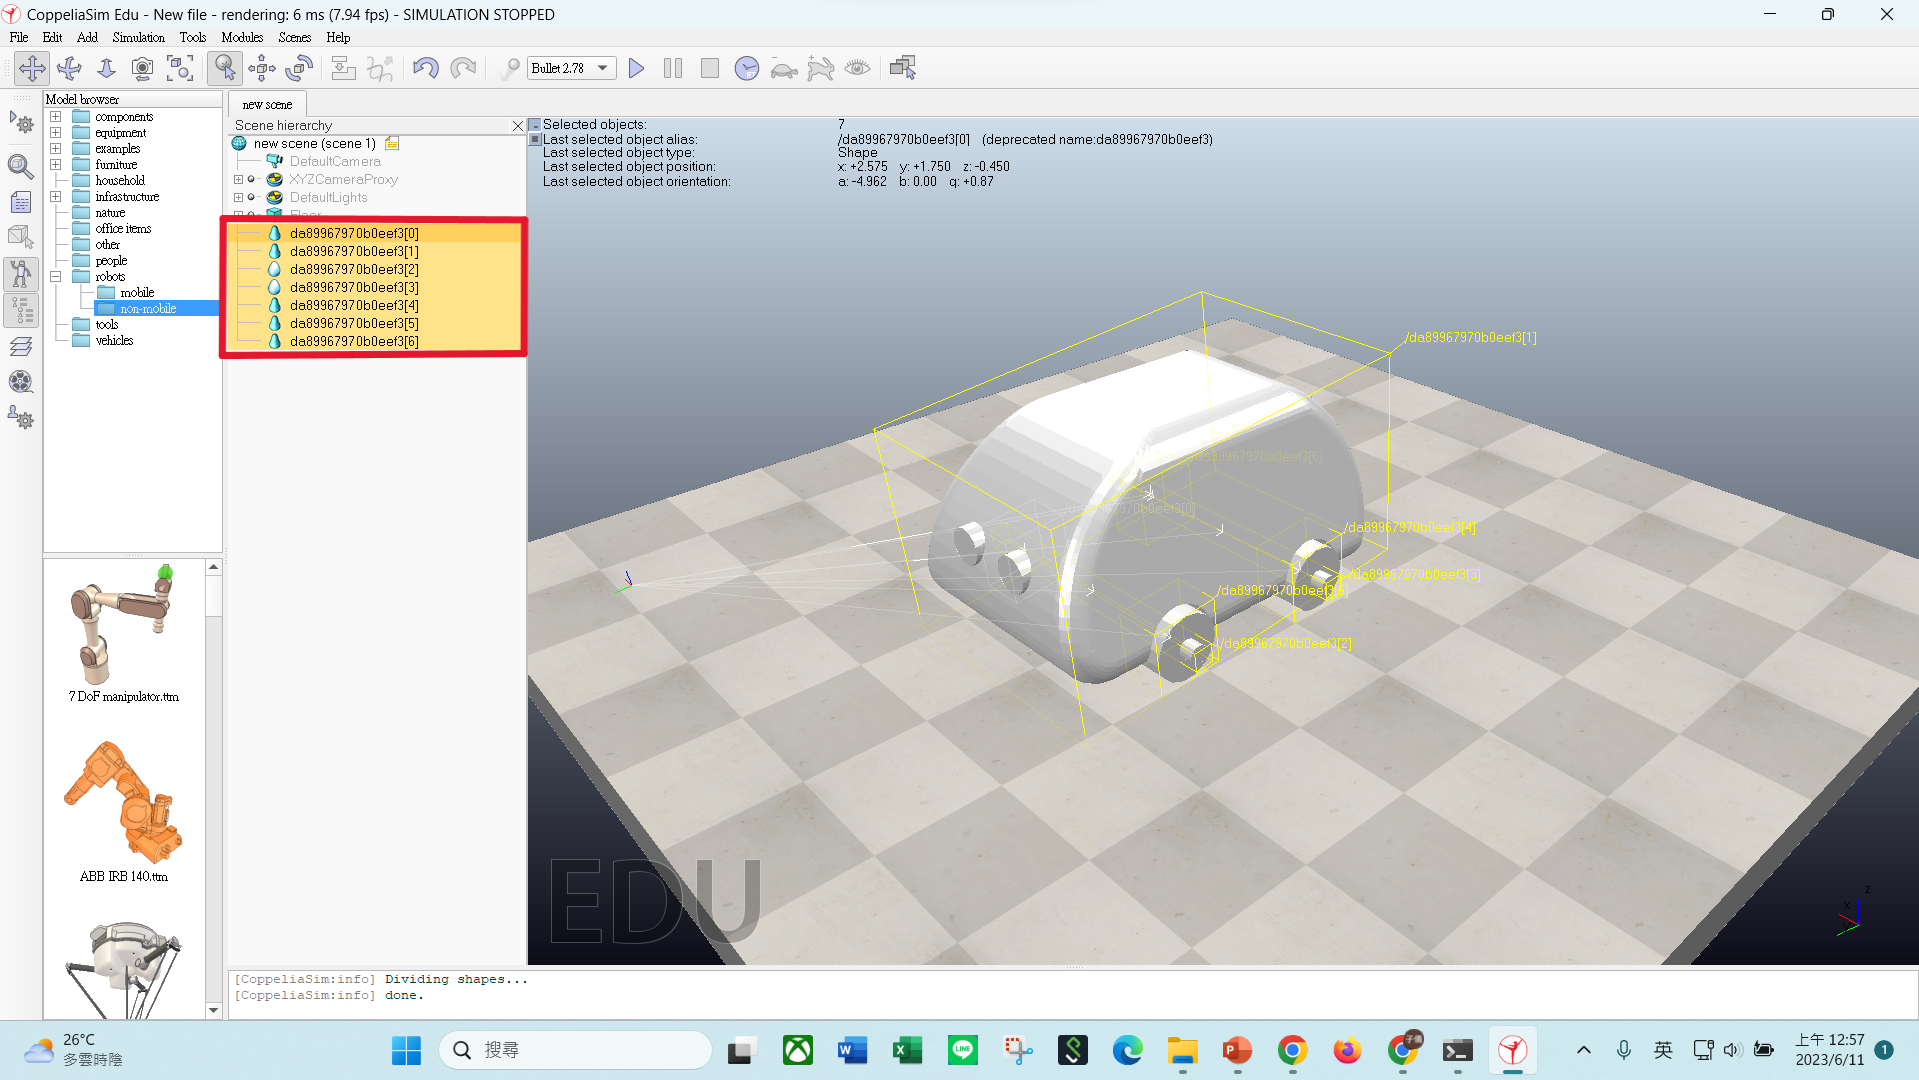
\includegraphics[width=0.5\textwidth]{球員組裝_2.png}
  \end{center}
  \caption{爆炸分解}
  \label{fig:photo}
\end{figure}

\begin{figure}[hbt!]
  \begin{center}
    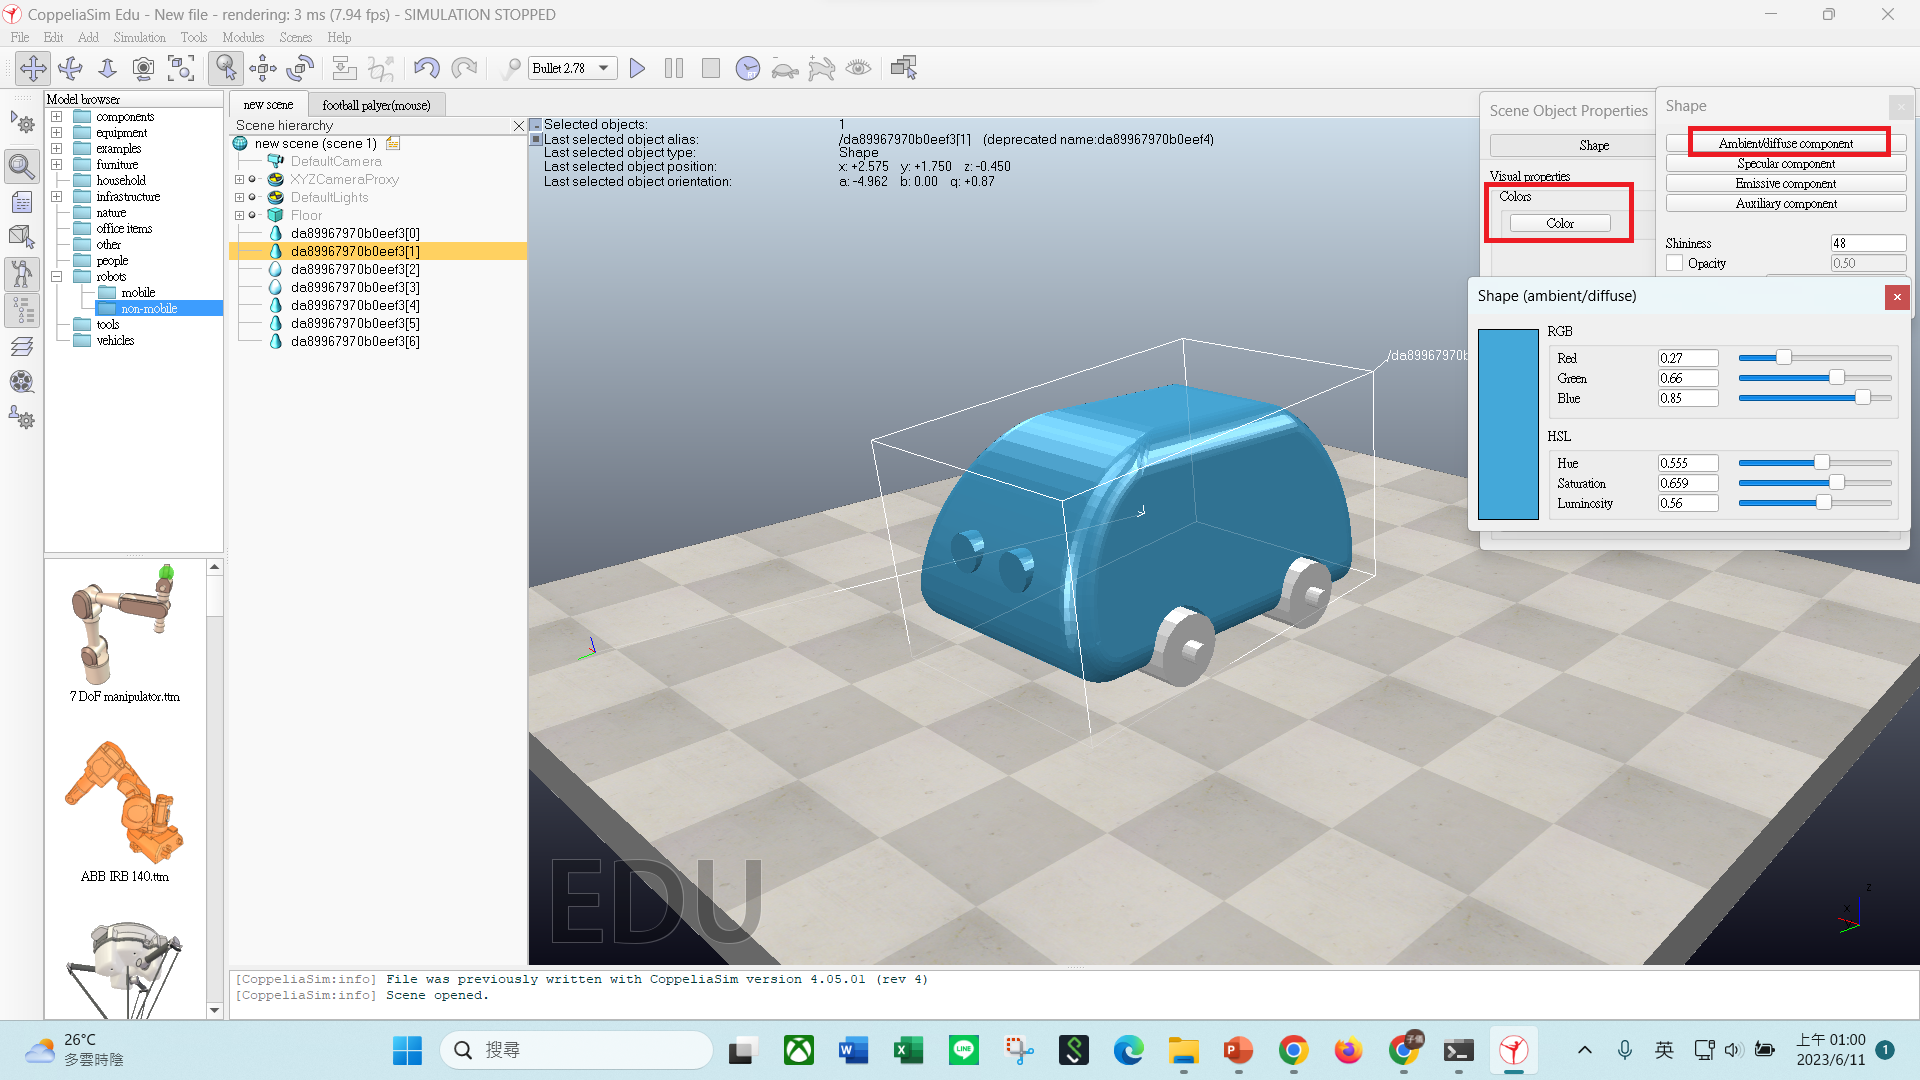
\includegraphics[width=0.5\textwidth]{球員組裝_3.png}
  \end{center}
  \caption{更改顏色}
  \label{fig:photo}
\end{figure}

\begin{figure}[hbt!]
  \begin{center}
    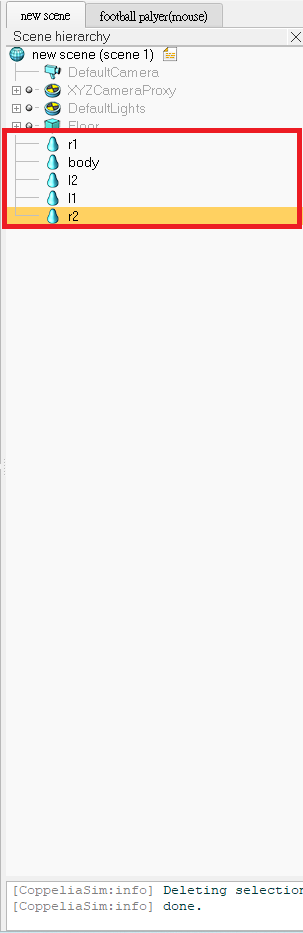
\includegraphics[width=0.5\textwidth]{球員組裝_4.png}
  \end{center}
  \caption{更改物件名稱}
  \label{fig:photo}
\end{figure}

\begin{figure}[hbt!]
  \begin{center}
    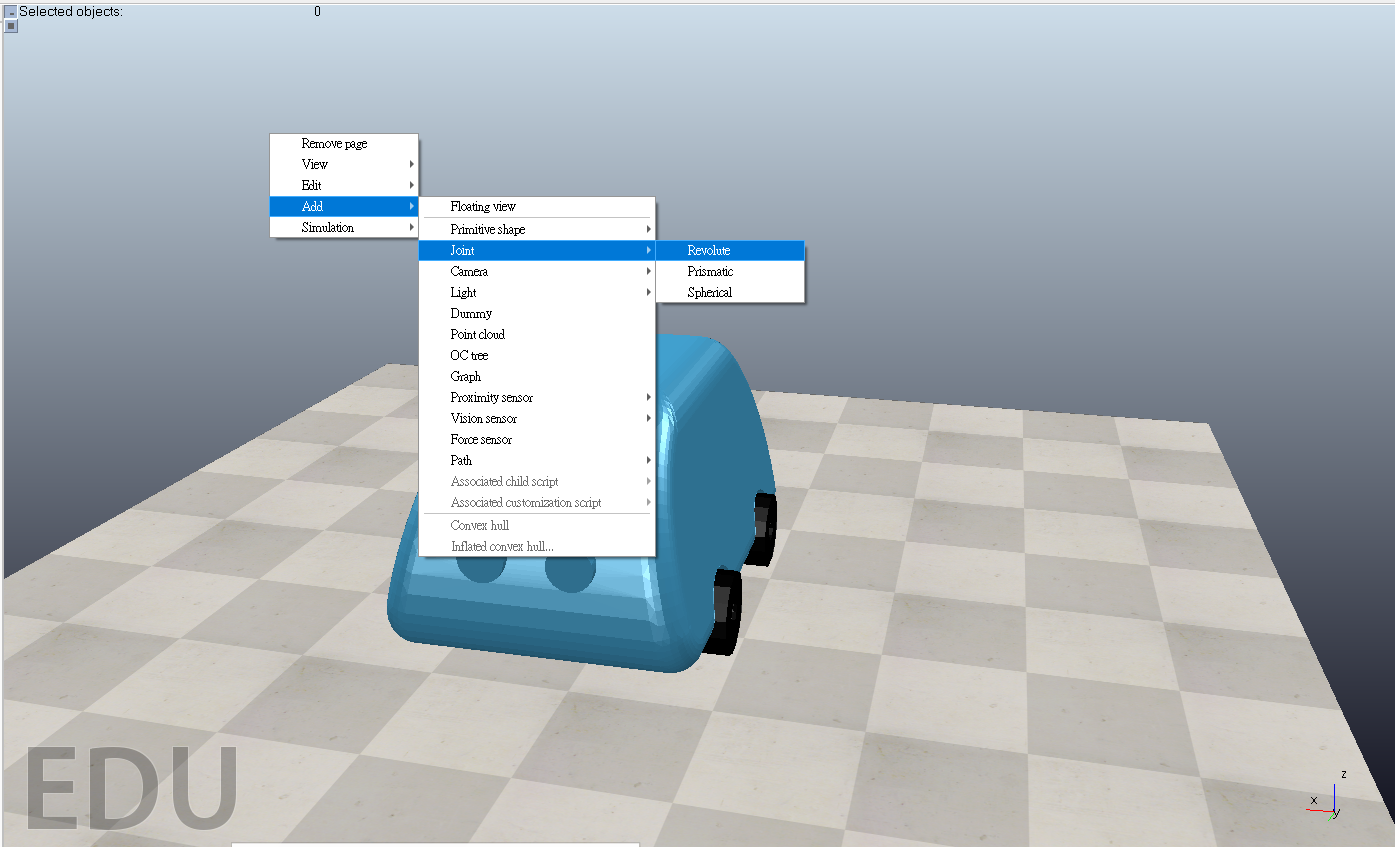
\includegraphics[width=0.5\textwidth]{球員組裝_5.png}
  \end{center}
  \caption{新增Joint}
  \label{fig:photo}
\end{figure}

\begin{figure}[hbt!]
  \begin{center}
    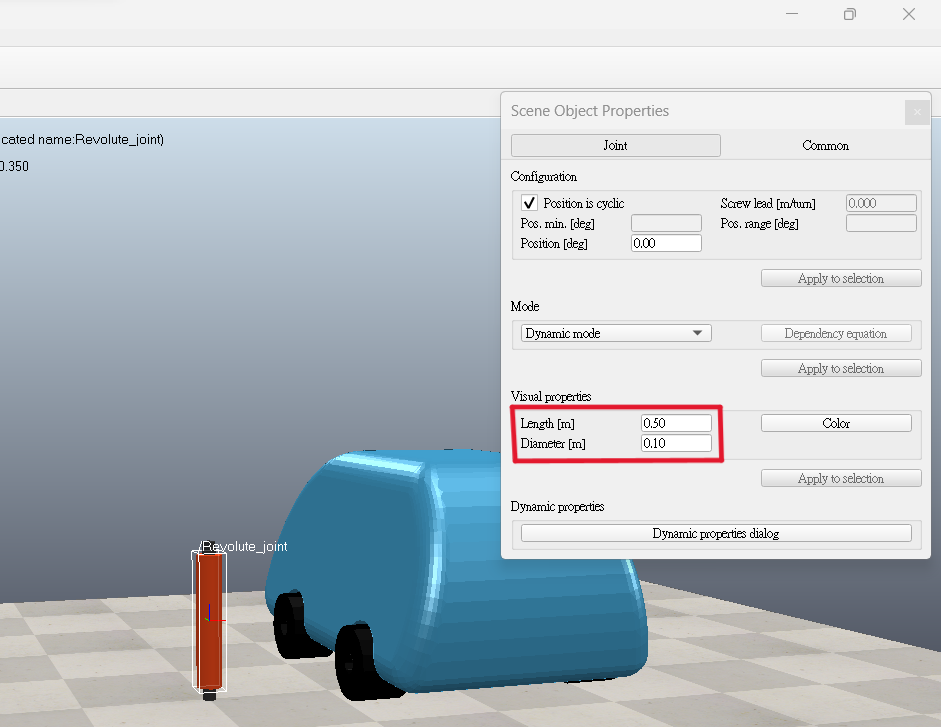
\includegraphics[width=0.5\textwidth]{球員組裝_6.png}
  \end{center}
  \caption{調整Joint大小}
  \label{fig:photo}
\end{figure}

\begin{figure}[hbt!]
  \begin{center}
    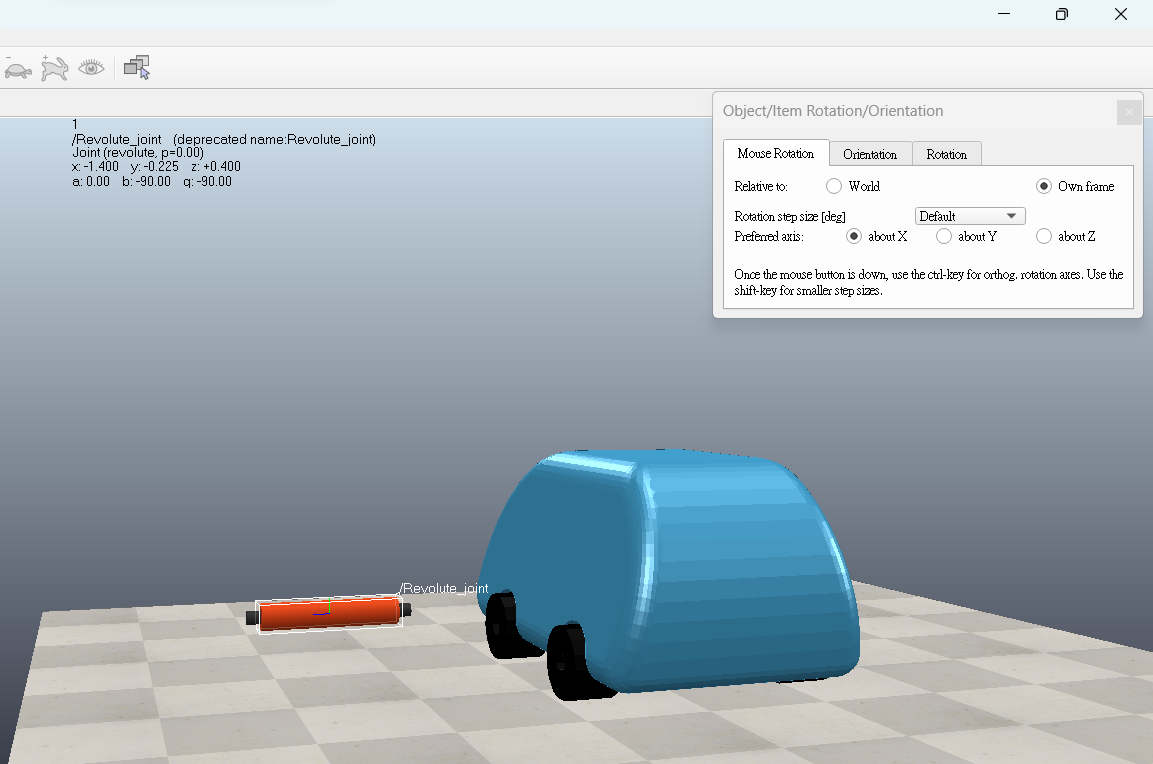
\includegraphics[width=0.5\textwidth]{球員組裝_7.png}
  \end{center}
  \caption{繞X軸旋轉,使Joint與物件平行}
  \label{fig:photo}
\end{figure}

\begin{figure}[hbt!]
  \begin{center}
    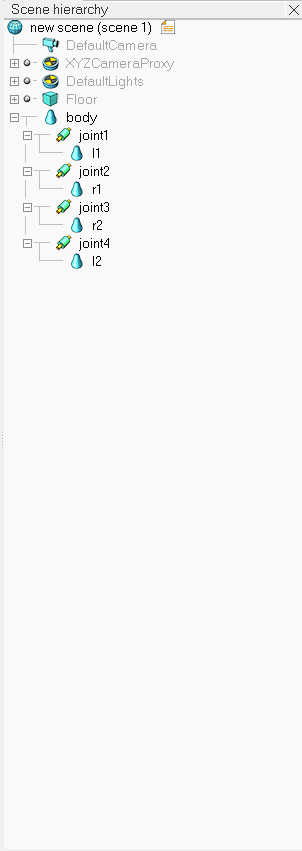
\includegraphics[width=0.5\textwidth]{球員組裝_8.png}
  \end{center}
  \caption{物件相互依附}
  \label{fig:photo}
\end{figure}

\begin{figure}[hbt!]
  \begin{center}
    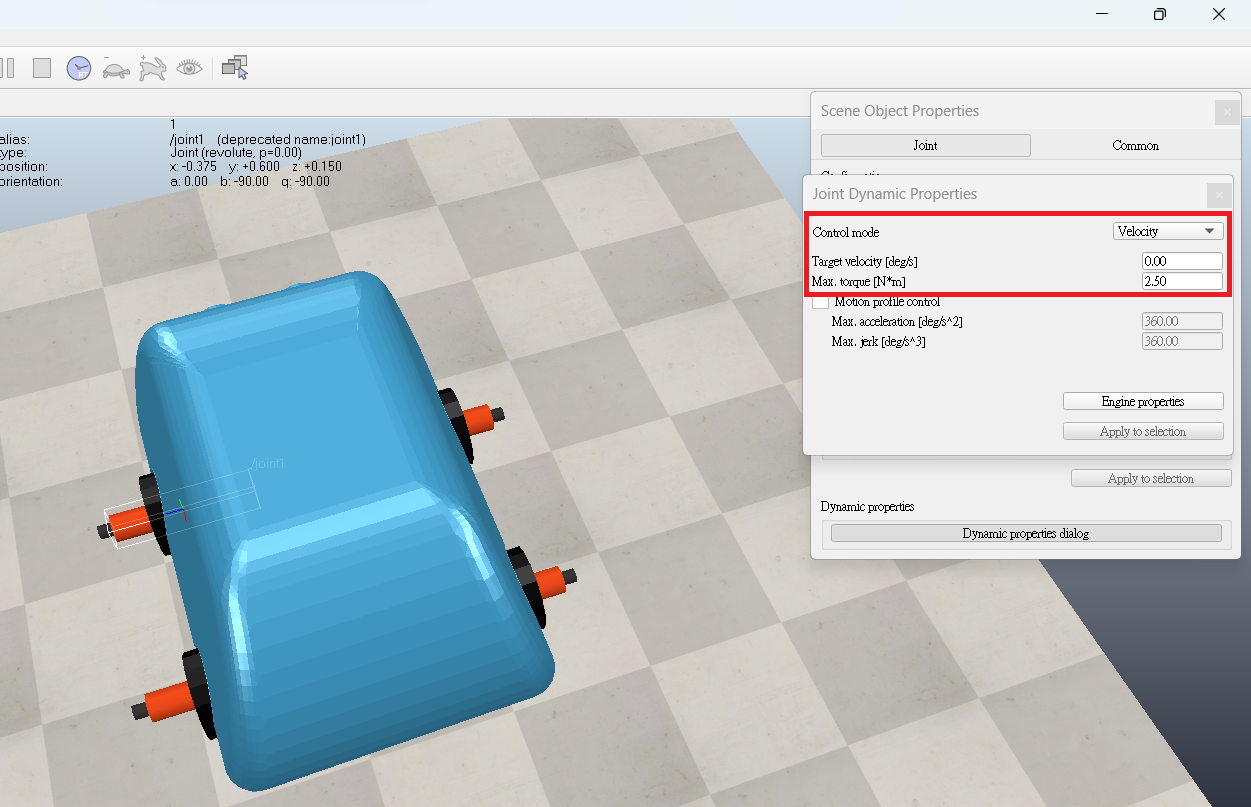
\includegraphics[width=0.5\textwidth]{球員組裝_9.png}
  \end{center}
  \caption{調整物件傳動參數}
  \label{fig:photo}
\end{figure}

\begin{figure}[hbt!]
  \begin{center}
    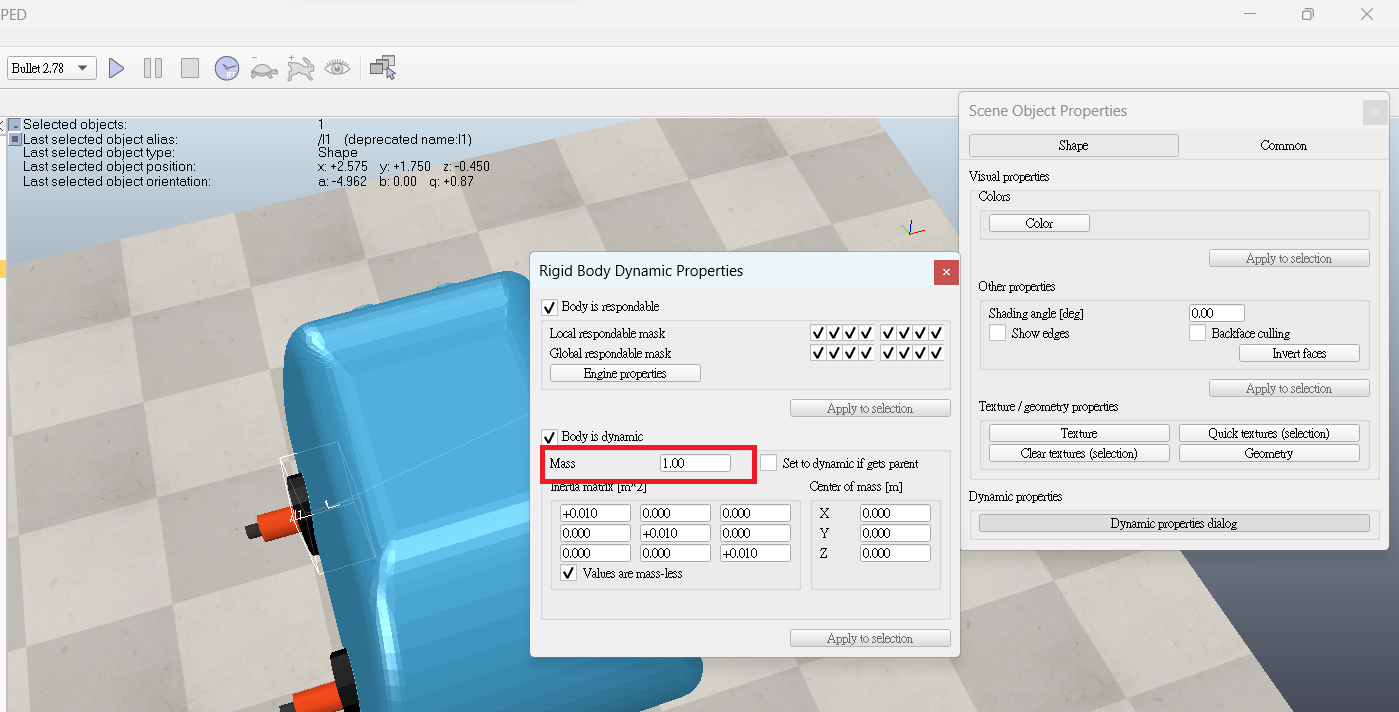
\includegraphics[width=0.5\textwidth]{球員組裝_10.png}
  \end{center}
  \caption{調整物件質量參數}
  \label{fig:photo}
\end{figure}

\newpage

\section{背號}
\begin{figure}[hbt!]
  \begin{center}
    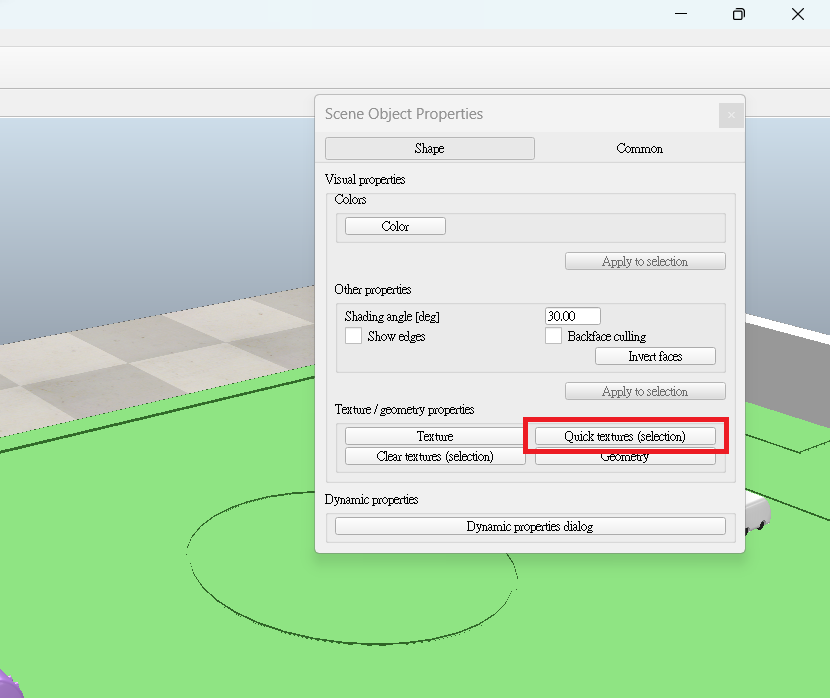
\includegraphics[width=0.5\textwidth]{球員背號_1.png}
  \end{center}
  \caption{變更物件材質(將數字貼在物件上)}
  \label{fig:photo}
\end{figure}
\begin{figure}[hbt!]
  \begin{center}
    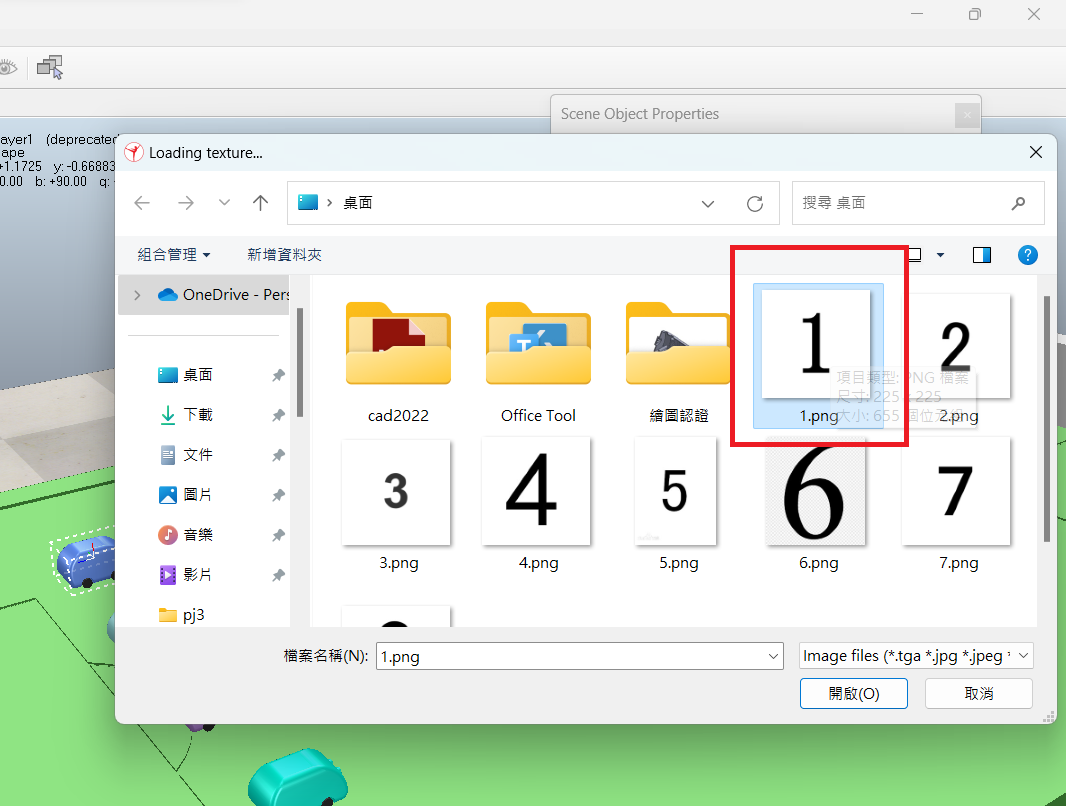
\includegraphics[width=0.5\textwidth]{球員背號_2.png}
  \end{center}
  \caption{選擇要使用的圖案}
  \label{fig:photo}
\end{figure}
\begin{figure}[hbt!]
  \begin{center}
    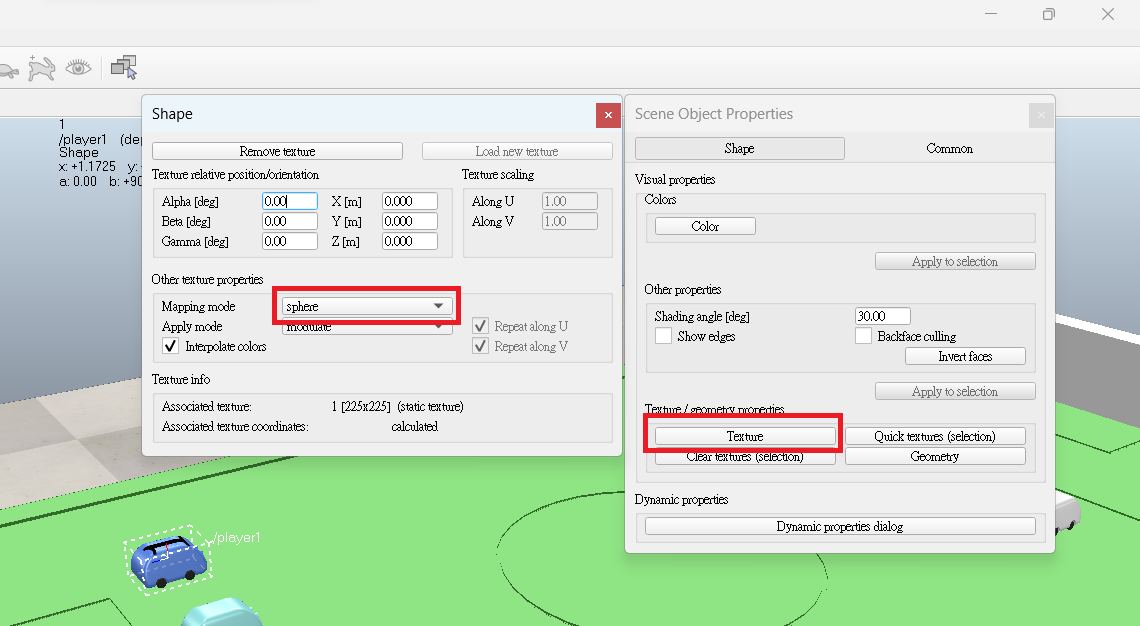
\includegraphics[width=0.5\textwidth]{球員背號_3.png}
  \end{center}
  \caption{調整映像參數}
  \label{fig:photo}
\end{figure}
\begin{figure}[hbt!]
  \begin{center}
    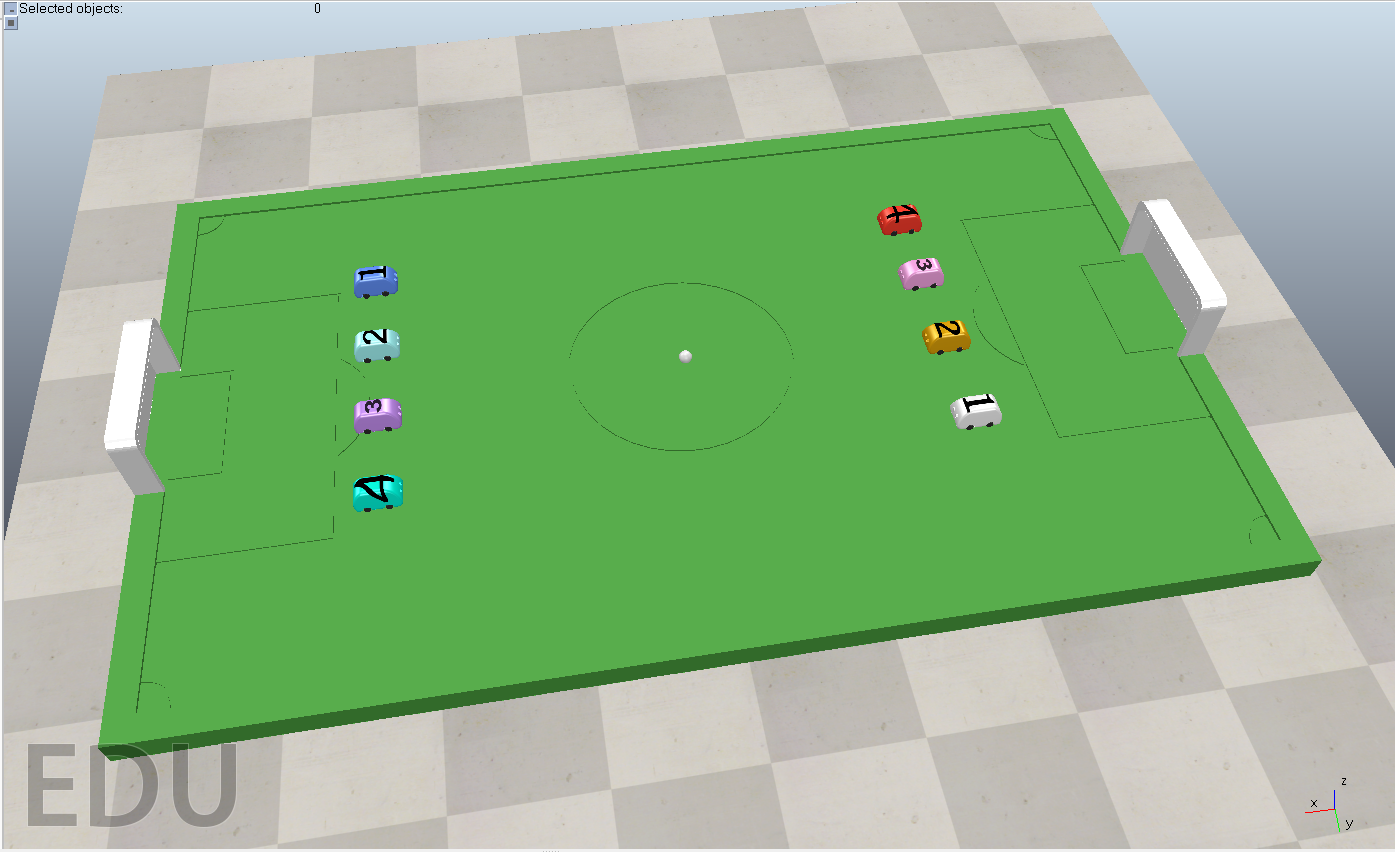
\includegraphics[width=0.5\textwidth]{球員背號_4.png}
  \end{center}
  \caption{背號完成}
  \label{fig:photo}
\end{figure}

\newpage

\section{程式碼}
連線主機---使用遠端 API 來連接到位於本地主機 (localhost) 上執行,RemoteAPIClient 是用於建立與遠端應用程式之間的通訊連接。指定了要連接的主機名稱為 "localhost" ,連接埠為 23000。使用 client.getObject("sim") 來獲取遠端應用程式中的一個名為 "sim" 的物件。 "Program started" 表示程式開始執行,然後程式執行 client.getObject("sim") 這行程式碼後,輸出了 "Simulation started" ,表示模擬 (simulation) 開始執行。
\begin{lstlisting}[language=Python, frame=single, numbers=left, captionpos=b, basicstyle=\ttfamily\small,showstringspaces=false, breaklines=true, tabsize=4, xleftmargin=15pt]
client = RemoteAPIClient('localhost', 23000)
print('Program started')
sim = client.getObject('sim')
#sim.startSimulation()
print('Simulation started')
\end{lstlisting}

輪子速度---定義一個 setBubbleRobVelocity 的函式,用於設定 BubbleRob 模型的輪子速度。首先使用 sim.getObject 函式獲取四個物件 leftMotor1、rightMotor1、leftMotor2、rightMotor2。用 sim.setJointTargetVelocity 函式 >>>設定輪子的目標速度,setJointTargetVelocity 函式 >>>設定 joint 的目標速度,因此可以用來控制輪子的運動。函式中的四個參數 leftWheelVelocity1、rightWheelVelocity1、leftWheelVelocity2、rightWheelVelocity2 分別代表四個輪子的速度。這些參數將會被傳遞給對應的 setJointTargetVelocity 函式來設定輪子的目標速度。
\begin{lstlisting}[language=Python, frame=single, numbers=left, captionpos=b, basicstyle=\ttfamily\small,showstringspaces=false, breaklines=true, tabsize=4, xleftmargin=15pt]
def setBubbleRobVelocity(leftWheelVelocity1, rightWheelVelocity1,leftWheelVelocity2, rightWheelVelocity2):
    leftMotor1 = sim.getObject('/lM1')
    rightMotor1 = sim.getObject('/rM1')
    leftMotor2 = sim.getObject('/lM2')
    rightMotor2 = sim.getObject('/rM2')
    sim.setJointTargetVelocity(leftMotor1, leftWheelVelocity1)
    sim.setJointTargetVelocity(rightMotor1, rightWheelVelocity1)
    sim.setJointTargetVelocity(leftMotor2, leftWheelVelocity2)
    sim.setJointTargetVelocity(rightMotor2, rightWheelVelocity2)
    #輸入四個變數分別給四個軸速度
\end{lstlisting}

輪子方向---定義名為 setBubbleRobangel 的函式。目的是根據輸入的參數 a,改變 BubbleRob 模型的前輪方向。首先使用 sim.getObject 函式獲取物件 bR,它代表 BubbleRob 模型的身體 (body)。接著程式計算出一個 angel 列表。angel 列表包含三個元素,第一個元素為 -90 度轉換為弳度的值,第二個元素為 a 度轉換為弳度的值,第三個元素為 0。然後用 sim.getObject 函式分別獲取物件 leftMotor 和 rightMotor,它們分別代表 BubbleRob 模型的左輪和右輪。最後使用 sim.setObjectOrientation 函式來設定物件的方向。該函式用於設定物件相對於參考物件的方向。在這裡將 leftMotor 和 rightMotor 的方向設定為相對於 bR 物件的方向,方向由 angel 列表指定。
\begin{lstlisting}[language=Python, frame=single, numbers=left, captionpos=b, basicstyle=\ttfamily\small,showstringspaces=false, breaklines=true, tabsize=4, xleftmargin=15pt]
def setBubbleRobangel(a):
    bR = sim.getObject('/bR')
    angel = [-90*math.pi/180, a*math.pi/180, 0]
    leftMotor = sim.getObject('/lM1')
    rightMotor = sim.getObject('/rM1')
    sim.setObjectOrientation(leftMotor, bR, angel)
    sim.setObjectOrientation(rightMotor, bR, angel)
    #輸入一個變數改變前輪方向
\end{lstlisting}

\newpage

控制---這段程式碼是一個無窮迴圈,它會持續監聽鍵盤的按鍵輸入,並根據按下的按鍵來控制 BubbleRob 模型的運動。目的是根據鍵盤輸入來控制 BubbleRob 模型的運動,並提供了前進、後退、旋轉和停止等功能。
\begin{lstlisting}[language=Python, frame=single, numbers=left, captionpos=b, basicstyle=\ttfamily\small,showstringspaces=false, breaklines=true, tabsize=4, xleftmargin=15pt]
while True:
    if keyboard.is_pressed('w'):
        setBubbleRobVelocity(4, 4, 4, 4)
        if keyboard.is_pressed('a'):
            setBubbleRobangel(-40)
        elif keyboard.is_pressed('d'):
            setBubbleRobangel(40)
        else:
            setBubbleRobangel(0)
    elif keyboard.is_pressed('s'):
        setBubbleRobVelocity(-4, -4, -4, -4)
        if keyboard.is_pressed('a'):
            setBubbleRobangel(-40)
        elif keyboard.is_pressed('d'):
            setBubbleRobangel(40)
        else:
            setBubbleRobangel(0)
    elif keyboard.is_pressed('a'):
        setBubbleRobVelocity(-4, 4, -4, 4)
    elif keyboard.is_pressed('d'):
        setBubbleRobVelocity(4, -4, 4, -4)
    elif keyboard.is_pressed('q'):
        % stop simulation
        sim.stopSimulation()
    else:
        setBubbleRobVelocity(0, 0, 0, 0)
        setBubbleRobangel(0)
#程式碼中使用 \text{keyboard.is_pressed} 函式來判斷指定的按鍵是否被按下。
#若按下 'w' 鍵,則呼叫 'setBubbleRobVelocity(4, 4, 4, 4)' 來設定 BubbleRob 模型的速度為正向,並根據 'a' 和 'd' 鍵的狀態設定前輪的方向。
#若按下 's' 鍵,則呼叫 'setBubbleRobVelocity(-4, -4, -4, -4)' 來設定 BubbleRob 模型的速度為負向,並根據 'a' 和 'd' 鍵的狀態設定前輪的方向。
#若按下 'a' 鍵,則呼叫 'setBubbleRobVelocity(-4, 4, -4, 4)' 來設定 BubbleRob 模型的速度使其向左旋轉。
#若按下 'd' 鍵,則呼叫 \textup{'setBubbleRobVelocity(4, -4, 4, -4)'} 來設定 BubbleRob 模型的速度使其向右旋轉。
#若按下 'q' 鍵,則停止模擬 (simulation)。
#若沒有按下任何按鍵,則呼叫 'setBubbleRobVelocity(0, 0, 0, 0)' 和 'setBubbleRobangel(0)',將 BubbleRob 模型的速度和前輪方向設定為零,即停止移動。
\end{lstlisting}
\newpage
